\documentclass{standalone}
\usepackage{tikz}
\begin{document}

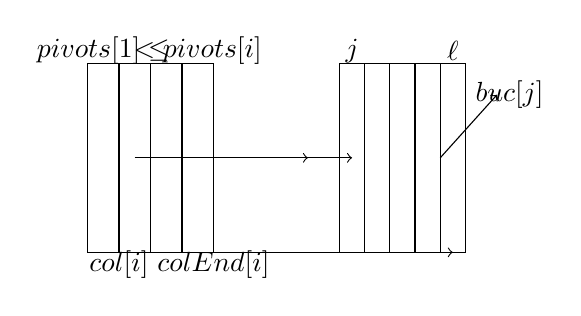
\begin{tikzpicture}[scale=0.8]
    % First matrix
    \draw (0,0) rectangle (2,3);
    \draw (0.5,0) -- (0.5,3);
    \draw (1,0) -- (1,3);
    \draw (1.5,0) -- (1.5,3);
    
    % Pointers and labels for first matrix
    \node at (0.25,3.2) {$\text{pivots}[1] \leq$};
    \node at (1.75,3.2) {$< \text{pivots}[i]$};
    \node at (0.5,-0.2) {$\text{col}[i]$};
    \node at (2,-0.2) {$\text{colEnd}[i]$};
    
    % Arrow between matrices
    \draw[->] (2.5,1.5) -- (3.5,1.5);

    % Second matrix
    \draw (4,0) rectangle (6,3);
    \foreach \x in {4, 4.4, 4.8, 5.2, 5.6} {
        \draw (\x,0) -- (\x,3);
    }
    
    % Pointers and labels for second matrix
    \node at (4.2,3.2) {$j$};
    \node at (5.8,3.2) {$\ell$};
    \draw[->] (5.6,1.5) -- (6.5,2.5);
    \node at (6.7,2.5) {$\text{buc}[j]$};

    % Connecting lines
    \draw[->] (0.75,1.5) -- (4.2,1.5);
    \draw[->] (2,0) -- (5.8,0);
\end{tikzpicture}

\end{document}